%%%%%%%%%%%%%%%%%%%%%%%%%%%%%%%%%%%%%%%%%%%%%%%%%%%%%%%%%%%%%%%%%%%%%
% LaTeX Template: Relatório de LSD
% Ano Letivo: 2026/2027
% Disciplina: Lógica e Sistemas Digitais
% Docente: Pedro Miguens Matutino
% Autor: Pedro Miguens Matutino
%%%%%%%%%%%%%%%%%%%%%%%%%%%%%%%%%%%%%%%%%%%%%%%%%%%%%%%%%%%%%%%%%%%%%%
\documentclass[12pt]{article}

\usepackage[a4paper]{geometry}
\usepackage[T1]{fontenc}
\usepackage[utf8]{inputenc}
\usepackage[portuguese]{babel}

\usepackage{graphicx, wrapfig, subcaption, setspace, booktabs}
\usepackage[font=small, labelfont=bf]{caption}
\usepackage{listings}
\usepackage{tocloft}
\usepackage{url, lipsum}
\usepackage{hyperref}

\usepackage{tikz}
\usetikzlibrary{karnaugh}

\usepackage{xcolor}
\usepackage{amsmath}
\usepackage{amsfonts}
\usepackage{amssymb}

\usepackage{enumitem}
\usepackage{algorithm}

\usepackage{fancyhdr}

%-------------------------------------------------------------------------------
% Definição da listagens de VHDL  ----------------------------------------------
%-------------------------------------------------------------------------------
\definecolor{vhdlkeyword}{RGB}{0,70,140}
\definecolor{vhdltype}{RGB}{130,0,80}
\definecolor{vhdlcomment}{RGB}{0.07,0.65,0.28}
\definecolor{vhdlstring}{RGB}{160,80,0}

\lstdefinelanguage{VHDL}{
    morekeywords={
        library,use,all,entity,is,port,in,out,inout,
        architecture,of,begin,end,signal,constant,
        component,configuration,package,body,
        process,wait,on,until,for,
        if,then,else,elsif,case,when,
        loop,while,next,exit,
        generate,generic,map,
        function,procedure,return,
        variable,file,type,subtype,record,array,
        downto,to,range,
        assert,report,severity,
        after,transport,inertial,
        with,select,others
    },
    morekeywords=[2]{
        std_logic,std_logic_vector,
        bit,bit_vector,
        integer,natural,positive,
        boolean,character,string,time
    },
    sensitive=true,
    morecomment=[l]--,
    morestring=[b]"
}

\lstset{
    language=VHDL,
    basicstyle=\ttfamily\tiny,
    keywordstyle=\color{vhdlkeyword}\bfseries,
    keywordstyle=[2]\color{vhdltype},
    commentstyle=\color{vhdlcomment}\itshape,
    stringstyle=\color{vhdlstring},
    numbers=left,
    numberstyle=\tiny\color{gray},
    numbersep=8pt,
    frame=single,
    breaklines=true,
    showstringspaces=false
}




\addto\captionsportuguese{
    \renewcommand{\figurename}{Figura}
    \renewcommand{\tablename}{Tabela}
    \renewcommand{\listfigurename}{Lista de Figuras}
    \renewcommand{\listtablename}{Lista de Tabelas}
}

% List of Figures
\renewcommand{\cftfigpresnum}{Figura~}
\renewcommand{\cftfigaftersnum}{}
\setlength{\cftfignumwidth}{5em}

% List of Tables
\renewcommand{\cfttabpresnum}{Tabela~}
\renewcommand{\cfttabaftersnum}{}
\setlength{\cfttabnumwidth}{5em}

% List of VHDL listings
\makeatletter
\renewcommand{\lstlistingname}{VHDL}
\renewcommand{\lstlistlistingname}{Lista de VHDL}
\renewcommand{\l@lstlisting}[2]{%
  \@dottedtocline{1}{0em}{5em}{VHDL~#1}{#2}%
}
\makeatother

%-------------------------------------------------------------------------------
% Início do documento ----------------------------------------------------------
%-------------------------------------------------------------------------------
 \begin{document}

% Parametros do documento
\tikzset{
  grp/.style n args={3}{
    draw=#1,fill=#1!30,
    minimum width=#2\kmunitlength,
    minimum height=#3\kmunitlength,
    rounded corners=0.2\kmunitlength,
    fill opacity=0.6,
    rectangle}
}
   
%-------------------------------------------------------------------------------
% Início da capa de rosto ------------------------------------------------------
%-------------------------------------------------------------------------------
\begin{titlepage}
    \begin{flushleft}
      \hspace{-1.5cm}
      
\includegraphics[height=3.5cm]{figures/01_ISEL-Logotipo-RGB_Horizontal-Compacto-900.png}

      Licenciatura em Engenharia Informática e de Computadores
    \end{flushleft}

    \vspace{2.0cm}

    \begin{center}
      \textbf{Lógica e Sistemas Digitais}

      2026 / 2027  inverno

      \vspace{0.5cm}
      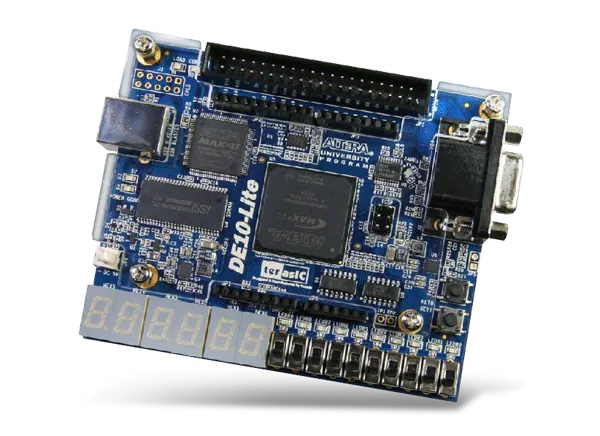
\includegraphics[width=6cm]{figures/de10-lite.jpg}\\
      \vspace{0.5cm}
      
      \Large {Relatório do \\Trabalho Laboratorial 1}\\
      
      \textbf{Circuitos Combinatórios}
    \end{center}

    \vspace{1.0cm}

Trabalho realizado por:

\begin{itemize}[label={}]
    \item Número Nome
    \item Número Nome
\end{itemize}

\vspace{0.5cm}
Turma:

Docente:

\date{}

\end{titlepage}
%-------------------------------------------------------------------------------
% Fim da capa de rosto ---------------------------------------------------------
%-------------------------------------------------------------------------------

%-------------------------------------------------------------------------------
% Parâmetros do cabeçalho e rodapé
%-------------------------------------------------------------------------------
\renewcommand{\headrulewidth}{1pt}
\definecolor{iselcolor}{rgb}{0.941,0.275 , 0.157} 
\definecolor{isel_beringela}{rgb}{0.37,0.08, 0.22} 
\renewcommand{\headrule}{\hbox to\headwidth{%
  \color{iselcolor}\leaders\hrule height \headrulewidth\hfill}}
\setlength\headheight{70pt}

\pagestyle{fancy}
\fancyhead{} % clear all header fields
\fancyhead[LO]{
\includegraphics[width=2.5cm]{figures/01_ISEL-Logotipo-RGB_Horizontal-Compacto-900.png}}
\fancyhead[RO]{\footnotesize Lógica e Sistemas Digitais 2025/2026 inverno \\ Trabalho Laboratorial 1}


%-------------------------------------------------------------------------------
% Indice, lista de figuras, lista de tabelas e lista de códigos
%-------------------------------------------------------------------------------
\setcounter{page}{1}
\pagenumbering{roman} % Roman page numbers
\tableofcontents
\clearpage
\addcontentsline{toc}{section}{\protect\numberline{}Lista de Figuras}
\listoffigures
\addcontentsline{toc}{section}{\protect\numberline{}Lista de Tabelas}
\listoftables
\addcontentsline{toc}{section}{\protect\numberline{}Lista de VHDL}
\lstlistoflistings
\clearpage

%-------------------------------------------------------------------------------
% Corpo do relatório
%-------------------------------------------------------------------------------
\pagenumbering{arabic} % Arabic/Indic page numbers
\setcounter{page}{1}

\section{Objetivo}
Qual o objetivo do projeto? Qual o assunto(s) a tratar.

\section{Descrição do Circuito a Projetar}
Descrever o problema (similar ao enunciado)

\section{Desenvolvimento do Projeto}
Descrever o desenvolvimento do projeto, incluindo a descrição do circuito, a função lógica, o diagrama de blocos, a simplificação lógica, a implementação em VHDL e a simulação.

\subsection{Diagrama de blocos}
Na Figura~\ref{fig:diagramablocos} ....
\begin{figure}[!h]
	\centering
	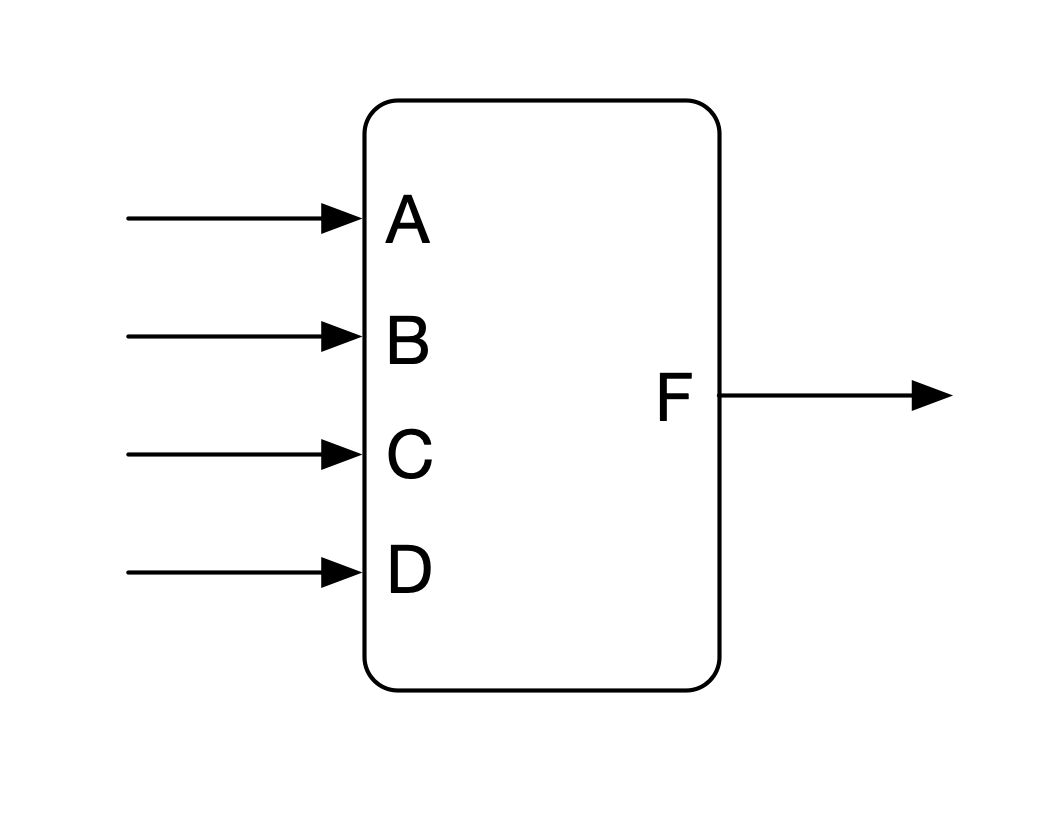
\includegraphics[width=0.5\textwidth]{figures/DiagramaBlocos.png}
	\caption{Diagrama de blocos da função F}
	\centering
	\label{fig:diagramablocos}
\end{figure}

\subsection{Funções lógicas dos circuitos}
Na equação~\eqref{eq:funcaoF} encontra-se ....
\begin{equation}
	f(A^+,B,C,D^-)=\sum{m(3,6,7,13,14,15)}+\sum{d(8,11,12)}
 \label{eq:funcaoF}
\end{equation}

\subsection{Simplificação lógica}
$f(A^+,B,C,D^-)=$
\begin{tikzpicture}[karnaugh,thick, enable indices]
  \karnaughmap{4}{}{{$A$}{$B$}{$C$}{$D$}}%
    {{}{}{}1{}{}11
    -{}{}--111}%
    {
      \node[grp={red}{1.9}{1.9}] at (3.0,2.0) {};
      \node[grp={blue}{1.9}{1.9}] at (2.0,2.0) {};
      \node[grp={green}{1.9}{1.9}] at (3.0,1.0) {};
    }
\end{tikzpicture}
$ = B \cdot C + A \cdot B +  C \cdot D $

Descreveu-se a função em VHDL, conforme~\ref{vhdl:ficheiro1}, utilizando~\cite{guiaQuartus}


\section{Resultados e Discussão}
Explicar o que foi feito para verificar a funcionalidade do circuito. Quais os resultados obtidos ...

\subsection{Simulação}
Realizou-se a simulação do circuito projetado conforme o ficheiro \textit{Testbench} descrito em VHDL~\ref{vhdl:ficheiro2} ...

\subsection{Teste}
Realizou-se o teste do circuito na placa DE10-lite, conforme a atribuição de pinos da Tabela~\ref{tab:pinos}.

\section{Conclusão} 
O trabalho consistiu em … \\
Foi desenvolvido em … \\ 
Foi testado na placa …\\
Os resultados experimentais confirmam o funcionamento do circuito de acordo com …

%-------------------------------------------------------------------------------
% REFERENCES
%-------------------------------------------------------------------------------
\clearpage
%\section*{Referências}
\addcontentsline{toc}{section}{\protect\numberline{}Referências}
\begin{thebibliography}{9}
\bibitem{guiaQuartus}
Pedro Miguens Matutino, Sérgio André \emph{Guia de Instalação do Quartus Prime Lite Edition 20.1.1.720}, 2022, ISEL.
\bibitem{de10liteManual}
Terasic \emph{DE10-lite User Manual}, 2020, Terasic.
\end{thebibliography}


\clearpage
\appendix
\section{VHDL}
% Inserção de ficheiro de descrição hardware
\lstinputlisting[
    caption={Descrição do circuito},
    label={vhdl:maioria}
]{vhdl/maioria.vhd}

% Inserção de ficheiro de descrição hardware
\lstinputlisting[
    caption={Testbench},
    label={vhdl:testbench}
]{vhdl/maioria_tb.vhd}


\clearpage
\section{Atribuição de Pinos}

\renewcommand{\arraystretch}{1.5}
\begin{table}[h]\footnotesize
	\caption{Atribuição de pinos para a função F~\cite{de10liteManual}}
  \centering
	\begin{tabular}{|l|c|}
	\hline
	\textbf{Entradas} & \textbf{pino} \\ \hline\hline
	A & C10  \\ 
	B & C11 \\
	C & D12 \\
	D & C12 \\ \hline \hline
	\textbf{Saídas} & \textbf{pino} \\\hline \hline
	F & A8  \\
	\hline
	\end{tabular}
	
	\label{tab:pinos}
\end{table}

\end{document}